%%%
% Automatic Layout
%%%

\section{Automatisches Layout}
\label{sec:automatic-layout}

% TODO: Verweis auf "graph-basierte Diagramme" in der Begriffsklärung
Den graph-basierten Softwarediagrammen unterliegt die abstrakte Struktur des Graphen (siehe Abschnitt X). Mit der graphischen Darstellung von Graphen beschäftigt sich die mathematische Disziplin des Graphzeichnens. Ihre Aufgabe besteht darin, Layout-Algorithmen zu entwerfen, die optimale Layouts in Hinsicht auf ästhetische Regeln erzeugen, d.h. die Layout-Eigenschaften wie Position der Knoten und Routen der Kanten berechnen \cite{Eichelberger05Aesthetics, Arvo02Techniques, Siebenhaller03Automatisches, Maier12A-Pattern-based}. Unter dem automatischen Layout für graph-basierte Diagramme sind daher vollautomatische Algorithmen zu verstehen, die für ein gegebenes Diagramm die optimalen Layout-Eigenschaften berechnen und das Diagramm entsprechend anpassen \cite{Fuhrmann11On-the-Pragmatics}.

Um während der Erstellung des Diagramms immer ein optimales Layout zu erhalten, muss der Layout-Algorithmus kontinuierlich nach jeder Änderung entweder automatisch oder manuell aufgerufen werden. Wenn eine Interaktion mit dem resultierenden Diagramm unterstützt wird, hat sie keinerlei Einwirkung auf den Algorithmus und wird bei dem nächsten Aufruf nicht berücksichtigt. In der Regel kann der Nutzer nur bestimmte Parameter des Algorithmus\footnote{z.B. minimale Länge der Kanten im zirkulären Layout-Algorithmus \lstinline{circo} aus der Bibliothek Graphviz \cite{NorthGansner14Dot-Manual}.} anpassen und hat somit nur einen geringen Einfluss auf das Ergebnis des Layout-Prozesses.

Die Ansätze lassen sich in zwei Kategorien nach der Art der Sprache unterteilen, die als Eingabe für den Layout-Algorithmus verwendet wird\footnote{In der Literatur werden Ansätze für das automatische Layout meistens nach den Layout-Algorithmen kategorisiert \cite[S.39ff]{Fuhrmann11On-the-Pragmatics}. In dieser Arbeit richtet sich die Kategorisierung danach, wie die Ansätze zu bedienen sind und welche Art der Interaktion sie unterstützen.}. Zu einem gibt es Ansätze, die aus einer Beschreibung des Diagramms in einer \textbf{textuellen Sprache} unter Anwendung des Layout-Algorithmus eine graphische Repräsentation erzeugen. Weiterhin gibt es Ansätze, die auf Diagramme angewendet werden, die in einer \textbf{visuellen Sprache} modelliert sind. Diese Ansätze verändern die Layout-Eigenschaften der Diagrammelementen direkt. Im Folgenden werden beide Kategorien behandelt.

% TODO: Visuelle Sprachen erklären, da [Fuhrmann] sagt, dass textuelle Sprachen auch visuelle Sprachen sind (S. 48)

\subsection{Textbasierte Ansätze}
\label{subsec:text-based-approaches}

Die textbasierten Ansätze für das automatische Layout erfordern als Eingabe eine textuelle Beschreibung des Diagramms, die in einer allgemeinen Auszeichnungssprache oder einer domänenspezifischen Sprache formuliert werden kann. Diese Beschreibung wird eingelesen und intern in ein abstraktes Modell umgewandelt, auf das der Layout-Algorithmus angewendet wird. Als Ausgabe wird eine statische Repräsentation des Diagramms in Form eines Bilds geliefert, die jegliche Möglichkeit der Interaktion vermisst. Durch die Entkopplung der Eingabe von der Ausgabe lässt sich das Diagramm nur durch eine Änderung des Quelltexts und einen wiederholten Aufruf des Layout-Algorithmus verändern.

\subsubsection{Graphviz}
\label{subsubsec:graphviz}

Es existiert eine Menge an Bibliotheken, die verschiedene Algorithmen für das Graphzeichnen implementieren\footnote{Insbesondere handelt es sich um hierarchische, kräftebasierte und orthogonale Algorithmen. \cite{Maier12A-Pattern-based}} und diese Funktionalität für andere Programme bereitstellen. Beispiele für solche Bibliotheken sind Graphviz\footnote{\url{http://graphviz.org}}, yFiles\footnote{\url{http://www.yworks.com/en/products_yfiles_about.html}} oder Kieler\footnote{\url{http://www.informatik.uni-kiel.de/en/rtsys/kieler/}} \cite{Maier12A-Pattern-based}. In dieser Arbeit wird Graphviz näher vorgestellt und insbesondere werden seine Aspekte des textbasierten und visuellen Ansatzes gezeigt.

Graphviz ist ein in der Programmiersprache C geschriebenes Tool für die Visualisierung von Graphen und wurde ursprünglich von AT\&T entwickelt. Es besteht aus folgenden Komponenten:

\begin{itemize}
    \item Domänenspezifische \textbf{Sprache Dot}\footnote{Der Aufbau der Sprache wird unter \url{http://www.graphviz.org/content/dot-language} erläutert. Ein Beispiel der Beschreibung eines Graphen ist im Quelltext \ref{lst:graphviz-dot-example-dot} gegeben.} für die Beschreibung von Graphen.
    % TODO: Bessere Beschreibung von verfügbaren Algorithmen
    \item Ein Satz von \textbf{Layout-Algorithmen}: u.a. \textit{dot}, \textit{neato}, \textit{fdp} oder \textit{circo} \cite{Gansner14Using, NorthGansner14Dot-Manual}
    \item Eine \textbf{Software-Bibliothek}, die die Funktionalität der Layout-Algorithmen und der graphischen Ausgabe bereitstellt und sich in andere Programme einbinden lässt \cite{Gansner14Using}.
    \item Ein Satz von \textbf{Kommandozeilen-Tools} für die Anwendung der Layout-Algorithmen und für die grafische Ausgabe \cite{NorthGansner14Dot-Manual}.
    \item Eine \textbf{GUI-Anwendung}, die über die selben Funktionen verfügt wie die Kommandozeilen-Tools.
\end{itemize}

% TODO: Algorithmen vorstellen?

Um einen Layout-Algorithmus auf einen Graph mit Hilfe der Komandozeilen-Tools oder der GUI-Anwendung anwenden zu können, muss der Graph in der Sprache Dot beschrieben werden. Ein Beispiel eines einfachen Graphen mit 4 Knoten und 3 Kanten ist im Quelltext \ref{lst:graphviz-dot-example-dot} gegeben.

\lstinputlisting[
    caption={Beschreibung eines Graphen in Dot (\lstinline{graphviz-dot-example.dot})},
    label={lst:graphviz-dot-example-dot}
]{resources/graphviz-dot-example.dot}

Mit dem Aufruf des Befehls aus dem Quelltext \ref{lst:grapviz-dot-example-sh} wird die oben aufgelistete Dot-Quelldatei \lstinline{graphviz-dot-example.dot} eingelesen, der beschriebene Graph wird in Form eines internen Modells instanziiert und auf das Modell wird der Layout-Algorithmus \lstinline{dot} angewendet. Anschließend wird mit dem Renderer \lstinline{png} ein Resultat in der PNG-Datei \lstinline{graphviz-dot-example.png} erzeugt, das in Abbildung \ref{fig:graphviz-dot-example} dargestellt ist \cite{Gansner14Using}.

\lstinputlisting[
    caption={Aufruf des Kommandozeilen-Tools \lstinline{dot}},
    label={lst:grapviz-dot-example-sh}
]{resources/graphviz-dot-example.sh}

\begin{figure}[hbt]
    \centering
    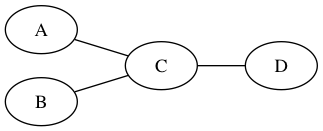
\includegraphics[scale=0.75]{resources/graphviz-dot-example.png}
    \caption{Resultat des Aufrufs des Kommandozeilen-Tools \lstinline{dot}}
    \label{fig:graphviz-dot-example}
\end{figure}

Alternativ kann die Dot-Quelldatei in der GUI-Anwendung geöffnet werden. In dem Fall wird das Ergebnis nicht direkt in eine Datei gespeichert, sondern als PDF in einem Fenster der Anwendung angezeigt.

In dem oben diskutierten Beispiel wird sichtbar gemacht, dass das resultierende Diagramm nicht interaktiv ist. Eine Änderung des Graphen ist nur in der Quelldatei möglich und ist mit einem wiederholten Aufruf des Kommandozeilen-Tools oder Laden der Datei in der GUI-Anwendung verbunden. Diese Schwachstelle wird durch 3rd-Party Editoren mit der integrierten graphischen Ausgabe wie etwa Leonhard\footnote{Leonhard ist ein graphischer Editor für Graphviz, der unter älteren Versionen von Mac OS X funktioniert. Weitere Information sind unter \url{http://algorithmique.net/leonhard.html} und \url{https://github.com/glejeune/Leonhard} zu finden.} oder WebGraphviz\footnote{\url{http://webgraphviz.com}} verbessert. In Leonhard wird die Übersetzung nach jeder Änderung des Quelltexts sogar automatisch gestartet.

Trotz der fehlenden Interaktivität des resultierenden Diagramms kann das Layout von dem Nutzer beeinflusst werden, indem der Layout-Algorithmus gewählt wird bzw. seine Parameter in der Quelldatei angepasst werden \cite{NorthGansner14Dot-Manual}. Im oben genannten Beispiel wurde der Layout-Algorithmus \lstinline{dot} verwendet und die Richtung des Graphen in der Dot-Quelldatei mit dem Befehl \lstinline{rankdir = LR} angepasst, so dass der Graph von links nach rechts gezeichnet wird.

\subsubsection{Textbasierte UML-Tools}

Neben den textbasierten Tools für das Graphzeichnen gibt es Tools, die für spezifische Domänen ausgelegt sind. Im Folgenden werden 2 textbasierte UML-Tools kurz vorgestellt, die aus einer textuellen Beschreibung in einer speziellen Sprache grafische UML-Diagramme erzeugen. Für die Berechnung des Layouts benutzen beide Tools intern die oben genannte Bibliothek Graphviz.

\paragraph{PlantUML}

\hyphenation{PlantUML}

PlantUML\footnote{\url{http://plantuml.sourceforge.net}} ist eine Java-Bibliothek, die für die Beschreibung von UML-Diagrammen die gleichnamige Sprache verwendet. Diese Sprache wird näher in \cite{Roques10Drawing} behandelt. Neben den vielen Anwendungen\footnote{Die bekannten Anwendungen sind unter \url{http://plantuml.sourceforge.net/running.html} aufgelistet.} bietet PlantUML einen Online-Editor\footnote{PlantUML Server: \url{http://www.plantuml.com/plantuml}} an, der es ermöglicht, UML-Diagramme direkt im Browser zu erzeugen und als Bilder zu exportieren.

\paragraph{yUML}

yUML\footnote{\url{http://yuml.me}} ist ein Online-Editor zum Erstellen von UML-Diagrammen im Browser. Im Unterschied zu PlantUML verwendet yUML eine anschauliche zeichenbasierte Sprache\footnote{Eine Übersicht der Syntax für Klassendiagramme: \url{http://yuml.me/diagram/scruffy/class/samples}}. Die Eingabe erfolgt über ein Textfeld und wird kontinuierlich in ein Bild übersetzt, das jederzeit exportiert werden kann. Alternativ wird eine URL-Adresse auf das Diagramm generiert \cite{Fuhrmann11On-the-Pragmatics}.

\subsubsection{Spezielle Algorithmen für Klassendiagramme}

% TODO: Speziellen Algorithmen ergänzen!

% Traditionelle Kriterien für Graphzeichnen sind für Klassendiagramme nicht ausreichend [Eichelberger S.79]

% SugiBib - ein Framework, das auf dem Sugiyama Algorithmus basiert und die Semantik und Strukturregeln berücksichtigt
% https://wwwi2.informatik.uni-wuerzburg.de/SugiBib
% XMI

% Kandinsky (Eiglsperger)

\subsection{Visuelle Ansätze}
\label{subsec:visual-approaches}

Die visuellen Ansätze für das automatische Layout unterscheiden sich von den textbasierten darin, dass der Layout-Algorithmus auf eine visuelle Sprache angewendet wird und dass das berechnete Layout direkt die Eingabe verändert. Diese Ansätze werden in der Regel in visuellen Editoren eingesetzt, die eine unmittelbare Bearbeitung des Diagramms unterstützen.

Der Ablauf ist wie folgt: Zunächst wird ein Diagramm in einer bestimmten visuellen Sprache (z.B. ein Klassendiagramm in der Sprache UML) modelliert. Dann wird ein Layout-Algorithmus (in der Regel manuell) ausgeführt, der das neue Layout für alle Diagrammbestandteile berechnet. Anschließend wird das modellierte Diagramm dermaßen angepasst, so dass es das berechnete Layout annimmt.

Die Entkoppelung der Ein- und Ausgabe, wodurch sich die textuellen Ansätze auszeichnen (siehe Abschnitt \ref{subsec:text-based-approaches}), entfällt an dieser Stelle und da das resultierende Diagramm interaktiv bleibt, kann es durch den Nutzer weiterhin verändert bzw. erweitert werden. Um nach jeder Änderung des Diagramms ein automatisch berechnetes Layout zu erhalten, muss allerdings der Layout-Algorithmus jedesmal erneut gestartet werden.

% TODO: Das "mentale Modell" erklären oder verweisen
Die Algorithmen für das automatische Layout sind im Allgemeinen nicht ideal und die Nutzer neigen dazu, das berechnete Layout für persönliche Präferenzen anzupassen, um ein mentales Modell bzw. eine sekundäre Notation\footnote{Unter der sekundären Notation ist eine zusätzliche Bedeutung des Diagramms zu verstehen, die durch das Layout geschaffen wird \cite{SeyboldGlinz03An-Effective}.} zu verwalten. Alle nachträglich manuell getätigten Layout-Änderungen werden bei einem erneuten Aufruf des Layout-Algorithmus verworfen und somit steht der Nutzer vor der Entscheidung, ob er nach jedem Aufruf des Algorithmus die Anpassungen wiederholt durchführt oder auf das automatische Layout komplett verzichtet \cite[S.119ff]{Eiglsperger04Automatic}.

\subsubsection{Automatisches Layout in OmniGraffle}

% Graphviz Layout Engine (siehe Webseite)
% Automatisches Layout aktivieren, Auswahl des Algorithmus, Einstellung der Parameter
% Aufruf manuelle oder nach Hinzufügen/Löschen einer Kante
% Animation

% Wie im Abschnitt \ref{subsubsec:graphviz} beschrieben, bietet Graphviz eine Software-Bibliothek an, die in andere Tools eingebunden werden kann.

\subsubsection{Automatisched Layout in Visual Paradigm}

% Zusatzfunktion
% semantische Unterstützung fehlt
% manueller Aufruf [Fuhrmann]
% verschiedene Algorithmen -> nur Verbindungen vs. alles

% yEd?

\subsection{Eigenschaften und Vergleich}

% TEXTBASIERT
%Aus diesem Grund ist dieser Ansatz eher für das Einbinden in automatisierte Prozesse (z.B. Generieren von Diagrammen in der automatisierten Dokumentation mit Doxygen\footnote{\url{http://www.stack.nl/~dimitri/doxygen/manual/diagrams.html}}) oder Wiki-Seiten geeignet, als für die Nutzung in einer interaktiven Umgebung.

%Die Layout-Algorithmen berücksichtigen keine Layout-Präferenzen der Nutzer und 

% Interaktion mit dem Diagramm wird von dem Layout-Algorithmus nicht (berücksichtigt) => Zerstören des mentalen Modells

% Zusammenfassung
%% Verletzung der Semantik- und Strukturregeln durch die mathematischen Algorithmen
%% Interaktion im Vordergrund ist gewünscht
%% nicht geeignet für den Prozess des Zeichnens
%% Unterstützung der Diagrammtypen und deren Strukturregeln

%% Zerstören des mentalen Modells [Eiglsperger03 zitieren]
%% bei allgemeinen Algorithmen werden die Semantik- und Strukturregeln nicht berücksichtigt

%% Neuordnung des Layouts -> Zerstören der sekundären Notation [Seybold]

% Vorteile:
%% gute Ergebnisse für kleine und einfache Diagramme

% Nachteile:
%% fehlende Interaktion: Knopfdruck
%% Nutzer kann wenig beeinflussen
%% nicht für Änderungen geeignet -> Neustart
%% Semantik und Struktur...
%% berücksichtigen nicht die anwendugspezifische Einschränkungen [Gladisch]
%% Mangel an Möglichkeit der Kontrolle des Ergebnisses [Gladisch]
%% Nicht für interaktive Umgebung geeignet [Maier 2.4.1]

% Nachteile Textbasierte Ansätze:
% - fehlende Interaktion des Nutzers mit dem Diagramm
% - Veränderungen an einer anderen Stelle, keine unmittelbare Bearbeitung des Diagramms
% - geringer Einfluss auf das Layout

% textuelle Ansätze: Durch Tools interaktiv, aber an 2 Stellen!

%Die automatischen Layout-Algorithmen sind nicht für eine interaktive Umgebung geeignet. [Maier]

% nicht geeignet für Änderungen im Diagramm -> muss nochmal gestartet werden

% (deutet darauf hin, dass) -> nicht intuitiv

% im Unterschied zu [Eichelberger] beschäftigt sich diese Arbeit mit interaktiven Ansätzen, da automatisches Layout gegen Agile Modeling verstößt

% die Interaktion mit dem Diagramm fehlt (textbasierte und teilweise auch grafische)
% statisch, nicht dynamisch, nicht interaktiv

% herrausstellen
